\section*{Lecture 0: A Nonmeasurable Set}

Consider the following half-open bounded interval
\begin{figure}[h]
    \centering
    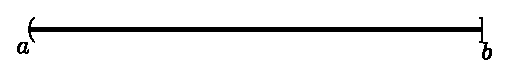
\includegraphics[scale=1.0]{Figures/half_open.eps}
    \caption{}
    \label{figure_1}
\end{figure}

Then the length of $(a,b]$ is $l((a,b])=b-a$. We can define the length of an
interval as a function $l:2^\R \xrightarrow{} \R^+_\infty$, where
$\R^+_\infty=\R^+ \cup \{\infty\}$. Notice then that the following hold for our
function $l$:
\begin{enumerate}
    \item[(1)] $l(A+y)=l(A)$, where $A+y=\{a+y : a \in A\}$.

    \item[(2)] If $A \subseteq B$, then  $l(A) \leq l(B)$.

    \item[(3)] For any collection $\{A_n\}$ of disjoint intervals, we have
        \begin{equation*}
            l(\bigcup{A_n})=\sum{l(A_n)}
        \end{equation*}
\end{enumerate}

Now, we wish to define a general function on all subsets of $\R$,  $\mu:2^\R
\xrightarrow{} \R^+_\infty$ such that
\begin{enumerate}
    \item[(1)] $\mu((a,b])=b-a$

    \item[(2)] If $A \subseteq B$, then  $\mu(A) \leq \mu(B)$.

    \item[(3)] $\mu(A+y)=\mu(A)$

    \item[(4)] For any disjoint collection of sets $\{A_n\}$,
        \begin{equation*}
            \mu(\bigcup{A_n})=\sum{\mu(A_n)}
        \end{equation*}
\end{enumerate}
We would also like $\mu(\emptyset)=0$.

\begin{theorem}\label{theorem_1}
    No such function $\mu:2^\R \xrightarrow{} \R^+_\infty$ satisfying (1)--(4)
    exists.
\end{theorem}
\begin{proof}
    Suppose such a function exists. Define the equivalence relation $\sim$ on
    $\R$ such that
    \begin{equation*}
        x \sim y \text{ if, and only if } x-y \in \Q
    \end{equation*}
    Let $\Lambda=\faktor{\R}{\sim}$. Then $\Lambda$ is not countable, as that
    would make $\R$ countable which is impossible. Now, let $R \subseteq [0,1]$
    a collections of representatives of equivalence classes of $\Lambda$, choose
    one representative for each element, by the axiom of choice, that is
    \begin{equation*}
    R=\{x : [x] \in \Lambda \text{ and } x=y \text{ if } [x]=[y]\}
    \end{equation*}
    Now, let $p,q \in \Q$, then we have that either  $R+p=R+q$ or that  $R+p$
    and  $R+q$ are disjoint. Suppose that they are not disjoint, and choose an
    $x \in (R+p) \cap (R+q)$. Then $x=\alpha+p$ and $x=\beta+q$. Thus
    $\alpha-\beta=q-p \in \Q$ which makes $\alpha \sim \beta$. By our
    definition, then  $\alpha=\beta$, and we get  $R+p=R+q$.

    Now consider the collection of all $\{R+q\}_{q \in \Q}$. This collection is
    disjoint as each $q$ is distinct, and consider
    \begin{equation*}
        \mu(\bigcup{R+q})=\sum{\mu(R+q)} \text{ for } -1<q<1
    \end{equation*}
    Notice that $\bigcup{R+q} \subseteq (-1,2)$, and so we get
    \begin{equation*}
        \sum{\mu(R+q)} \leq \mu((-1,2))=3 \text{ for } -1<q<1
    \end{equation*}
    By (3), we also get that
    \begin{equation*}
        \mu(R+q)=\mu(R)
    \end{equation*}
    so that
    \begin{equation*}
        \sum{\mu(R)} \leq \mu((-1,2))=3
    \end{equation*}
\end{proof}

Now, since this sum is bounded, $\mu(R)=0$. On the other hand, notice that
$(0,1) \subseteq \bigcup{R+q}$. So that $\mu((0,1))=1 \leq \mu(R)=0$. This is a
contradiction. Therefore no such $\mu$ exists.

\begin{definition}
    We call a set for which no such function $\mu$, satisfying (1)--(4) exists a
    \textbf{nonmeasurable set}.
\end{definition}

We would now like to restrict our sets to those that permit such a function
$\mu$ to exist; the so called ``measurable'' sets.
